\chapter{Numerical Simulations and Results \label{results}}
In this chapter we discuss the numerical results of the implementation of algorithm \ref{Algorithm} using the PyMongeAmpere library \cite{Merigot2017a} for solving the optimal transport problem. The use of this algorithm allows us to produce results with higher resolutions than previously realised. Plotting the Laguerre diagrams confirms the formation of a front as compared to similar results produced by \cite{Nakamura1994,Cullen1993}. Finally, the validity of the numerical implementation is investigated and performance analysed to assert the suitability of the numerical implementation in providing a solution to equations \ref{EadyModel}.
\section{Physical interpretation of Results \label{laguerre plots}}
Using the plotting process described in section \ref{plotting}. The Laguerre diagrams below show snapshots of frontogenesis and the subsequent evolution of the front. The model was initialised with a grid of $80 \times 40$ points taken from an optimised sampling of points in the physical domain $\Gamma = [-L,L]\times[0,H]$ and transformed to geostrophic co-ordinates as explained in \ref{Initpoints}. This involves an application of Lloyd's algorithm where first moments of cells are iteratively found until points are equidistant in the domain. A summary of parameter values in given in table \ref{param vals}.  For the following results Heun's method described in section \ref{Heun} was used for time-stepping for a time period of 25 days from a randomly generated mesh.
\\
\linebreak
\begin{table}
	\begin{tabular}{|c|c|c|c|}
		\hline 
		Parameter & Value & Parameter & Value \\
		\hline 
		$L$ & $1 \times 10^6 \ m$ & $H$ & $1 \times 10^4 \ m$ \\ 
		\hline 
		$g$ & $10 \ ms^{-2}$ &	$f$ & $10^{-4} \ s^{-1}$ \\ 
		\hline 
		$N^2$ & $2.5 \times10^{-5} \ s^{-2}$&$\theta_0$ & $300 \ K$ \\ 
		\hline 
		C & $3 \times 10^{-6} \ m^{-1}K$ & $B$ & $0.25 \ Ks^{-1}$ \\ 
		\hline 
	\end{tabular}
	\caption[Table of parameter values used in numerical implementation of SG/DA]{Table of parameter values used in numerical implementation of SG/DA as given by \cite{Cullen2006a} with $B$ chosen independently.}
	\label{param vals}
\end{table}
In diagrams \ref{fig: thetap ldiag1}-\ref{fig: thetap ldiag2} we see the growth of the normal mode instability. Initially (a) the stratification of potential temperature, $\theta '$ is linear, as in the base state. By $2.5$ (b) days we see the instability appear in the form of a wave and by $6$ days a strong front has formed as a large gradient in $\theta '$. We see that warmer air in the upper atmosphere has been come down into the lower regions of the atmosphere. By (d) the front has collapsed again as the normal mode instability loses its predominance. 
\\
\linebreak
An interesting phenomenon observed after this is that the instability grows again and a secondary front is formed. A cycle then forms of an growing instability in one direction forming a front which is then dissipated and a subsequent instability grows in the opposite direction. Some snapshots of this cycle are shown in the images below. This cycle is due to the balance between the normal mode instability and the background shear. Initially the instability is free to grow dominating the dynamics and leading to frontogenesis. The vertical shear counterbalances the growth of the instability dissipating the front. Internal instabilities then act to contribute towards the growth of a new front, however this secondary front is not as strong. The vertical shear again acts to restore the system to its original state and the cycle continues like this. 
\newpage
\begin{figure}[ht!]
	\centering
	\subfloat[]{{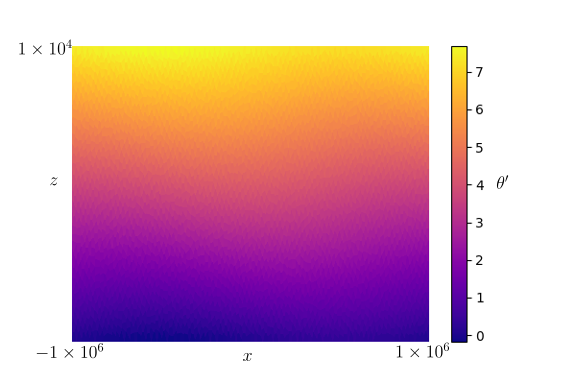
\includegraphics[width=0.9\linewidth]{evaluation/laguerre_diagram_thetap_0}}}\\
	\subfloat[]{{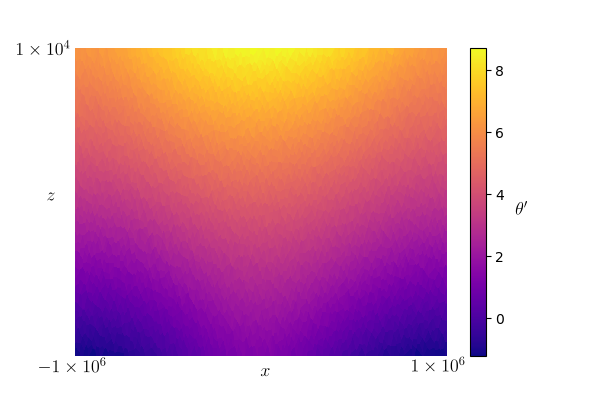
\includegraphics[width=0.9\linewidth]{evaluation/laguerre_diagram_thetap_5}}}
	\caption{Plots of Laguerre Diagrams shaded according to the value of $\theta '$ using a random mesh of $80 \times 40$ points initialised in geostrophic space using \ref{Initpoints} at (a) $0$ days, (b) $2.5$ days (c) $6$ days and (d) $9$ days, $\Gamma = [-L,L]\times[0,H]$, where $L = 1\times10^6$ and $H = 1\times10^4$}
	\label{fig: thetap ldiag1}
\end{figure}
\begin{figure}[ht!]
	\centering
	\subfloat[]{{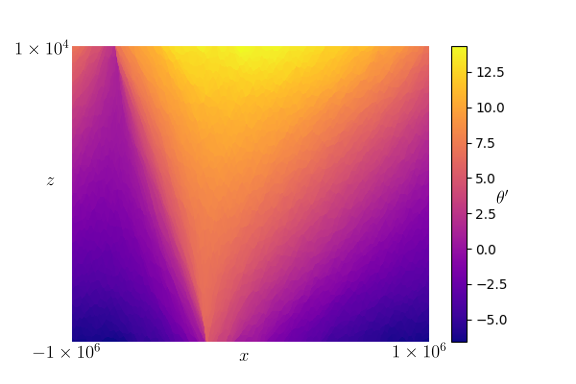
\includegraphics[width=0.9\linewidth]{evaluation/laguerre_diagram_thetap_12}}}\\
	\subfloat[]{{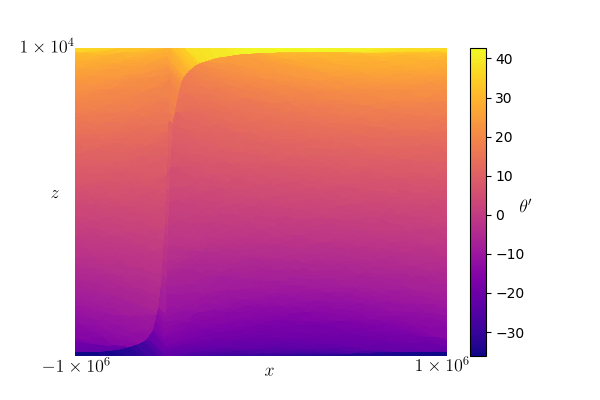
\includegraphics[width=0.9\linewidth]{evaluation/laguerre_diagram_thetap_18}}}\\
	\caption{Plots of Laguerre Diagrams shaded according to the value of $\theta '$ using a random mesh of $80 \times 40$ points initialised in geostrophic space using \ref{Initpoints} at (a) $6$ days, (b) $9$ days, $\Gamma = [-L,L]\times[0,H]$, where $L = 1\times10^6$ and $H = 1\times10^4$}
	\label{fig: thetap ldiag2}
\end{figure}
\newpage
Diagram (a) in \ref{fig: front_cycle} shows the formation of the secondary front, (b) \ref{fig: front_cycle}  in  shows its collapse and (c) shows the formation of a third front with a reversed gradient in $\theta '$. The front formation is not as clear in these images. The range in $\theta '$ has been reduced to half its original range to illustrate the cycle better. This leads to a saturation of colour at the top an bottom of the Laguerre diagrams as extreme values of $\theta '$ are mapped to the end points of the scale. As suggested by Dr Cotter this could be due to outlying points which contribute to extreme values of $\theta '$. This skews the colour range as seen in figure \ref{fig: front_cycle}
\begin{figure}[h!]
	\centering
	\subfloat[]{{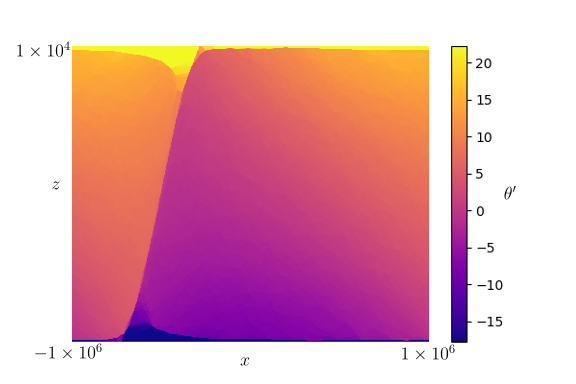
\includegraphics[width=0.6\linewidth]{evaluation/laguerre_diagram_thetap_22}}}\\
	\subfloat[]{{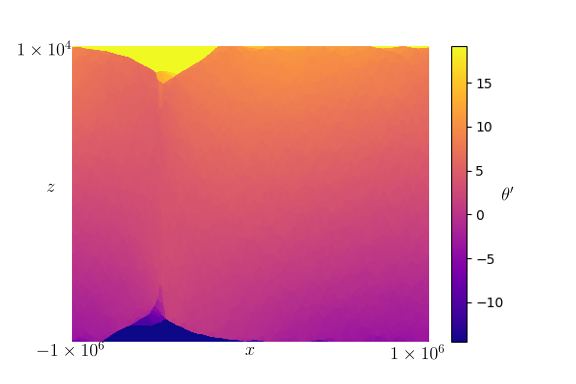
\includegraphics[width=0.6\linewidth]{evaluation/laguerre_diagram_thetap_25}}}\\
	\subfloat[]{{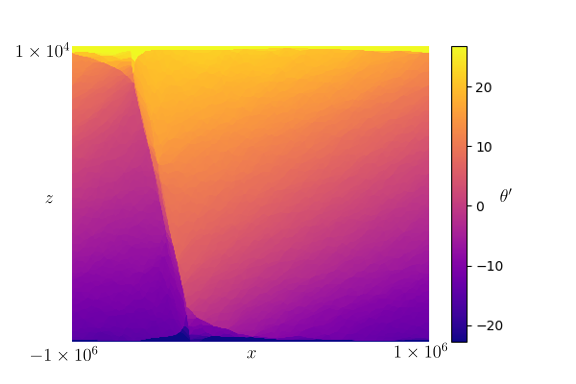
\includegraphics[width=0.6\linewidth]{evaluation/laguerre_diagram_thetap_29}}}\\
	\caption{Plots of Laguerre Diagrams shaded according to the value of $\theta '$ using a random mesh of $80 \times 40$ points initialised in geostrophic space using \ref{Initpoints} at (a) $11$ days, (b) $12.5$ days (c) $14.5$ days, $\Gamma = [-L,L]\times[0,H]$, where $L = 1\times10^6$ and $H = 1\times10^4$}
	\label{fig: front_cycle}
\end{figure}


\begin{figure}[ht!]
	\centering
	\subfloat[]{{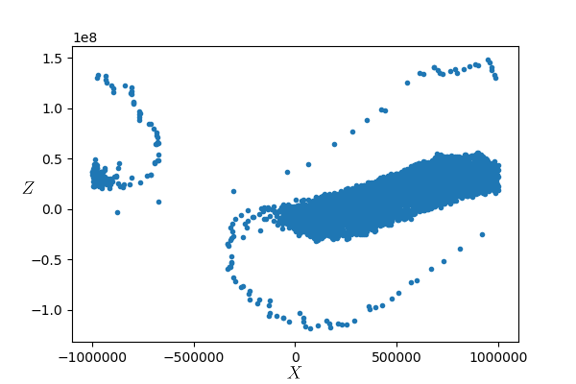
\includegraphics[width=0.6\linewidth]{evaluation/Gpoints_22}}\label{Gpoints_front11}}
	\caption{Plot of Geostrophic points at $11$ days}
	\subfloat[]{{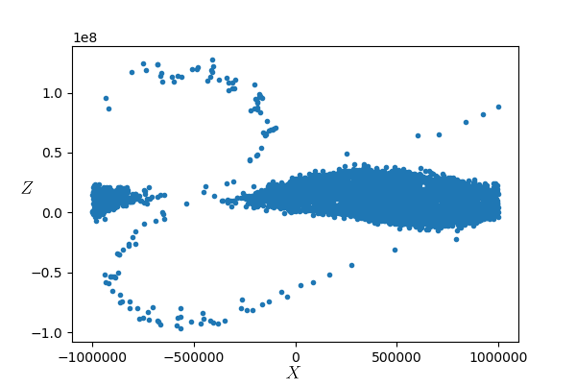
\includegraphics[width=0.6\linewidth]{evaluation/Gpoints_25}}\label{Gpoints_front12.5}}
	\caption{Plot of Geostrophic points at $12.5$ days}
	\subfloat[]{{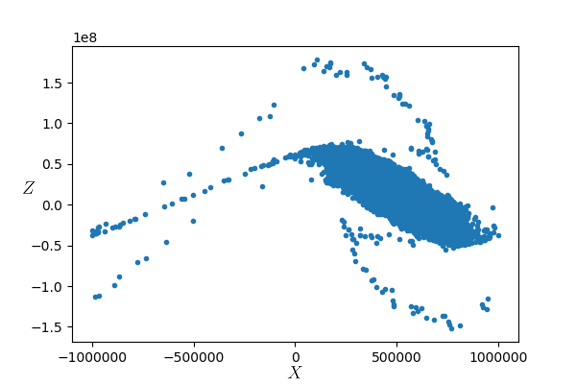
\includegraphics[width=0.6\linewidth]{evaluation/Gpoints_29}}\label{Gpoints_front14.5}}
	\caption{Plot of Geostrophic points at $14.5$ days}
\end{figure}

Another interesting visualisation of the result is that of using $v_g$ the cross slice velocity as a colour scale. The diagrams below illustrate this for the same data as in figures \ref{fig: thetap ldiag1}, \ref{fig: thetap ldiag2}. The front formation is a lot clearer in this case especially for the cycle of front formation and collapse.
\newpage
\begin{figure}[ht!]
	\centering
	\subfloat[]{{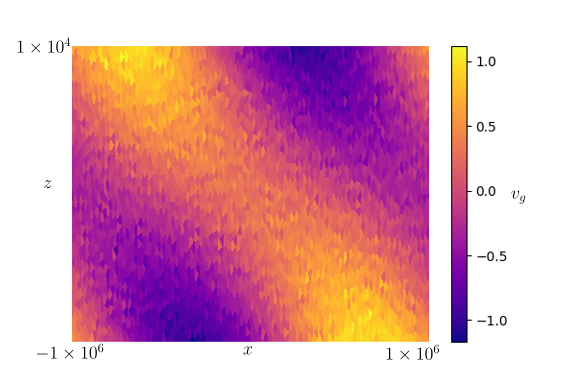
\includegraphics[width=0.7\linewidth]{evaluation/laguerre_diagram_vg_0}}}\\
	\subfloat[]{{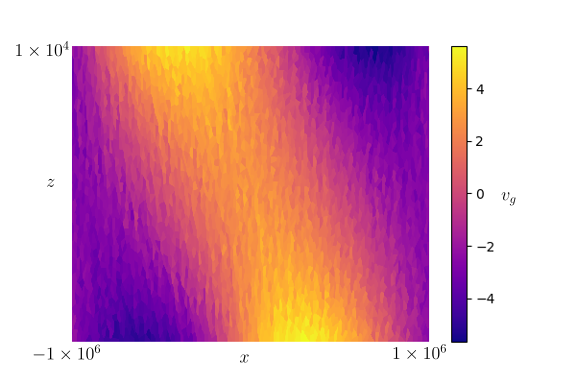
\includegraphics[width=0.7\linewidth]{evaluation/laguerre_diagram_vg_5}}}
	\caption{Plot of Laguerre Diagrams shaded according to the value of $v_g$ using a random mesh of $80 \times 40$ points initialised in geostrophic space using \ref{Initpoints} at (a) $0$ days and (b) $2.5$ days , $\Gamma = [-L,L]\times[0,H]$, where $L = 1\times10^6$ and $H = 1\times10^4$}
	\label{vg0}
\end{figure}
\newpage
\begin{figure}[h!]
	\centering
	\subfloat[]{{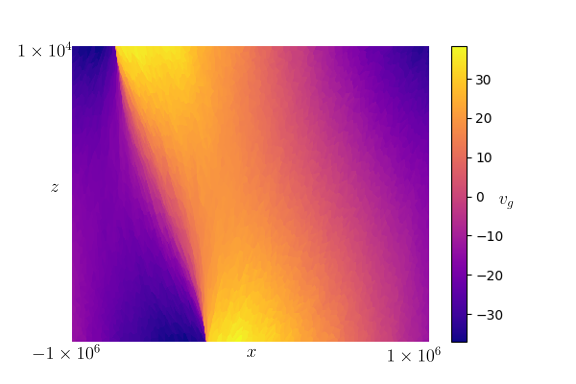
\includegraphics[width=0.7\linewidth]{evaluation/laguerre_diagram_vg_12}}}\\
	\subfloat[]{{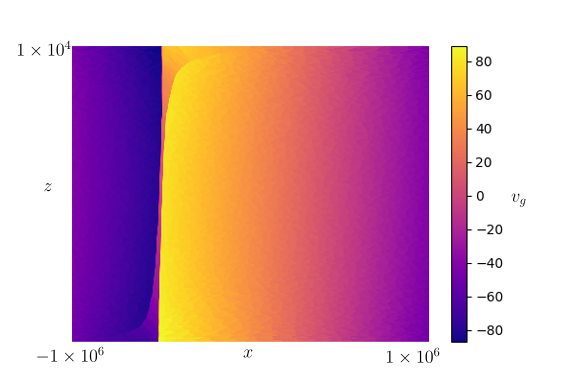
\includegraphics[width=0.7\linewidth]{evaluation/laguerre_diagram_vg_18}}}
	\caption{Plots of Laguerre Diagrams shaded according to the value of $v_g$ using a random mesh of $80 \times 40$ points initialised in geostrophic space using \ref{Initpoints} at (a) $6$ days (b) $9$ days $\Gamma = [-L,L]\times[0,H]$, where $L = 1\times10^6$ and $H = 1\times10^4$}
	\label{vg2.5}
\end{figure}
\begin{figure}[ht!]
	\centering
	\subfloat[]{{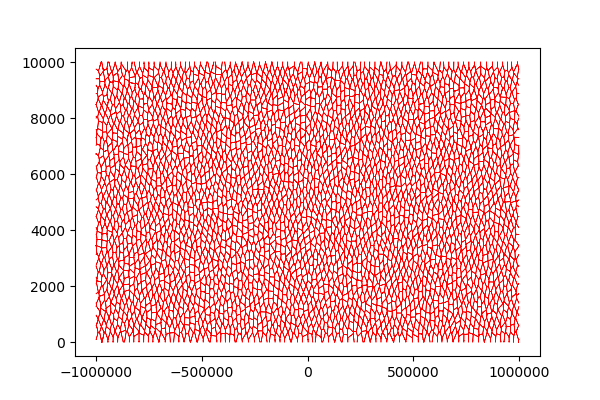
\includegraphics[width=0.7\linewidth]{evaluation/laguerre_tesselation_0}}}\\
	\subfloat[]{{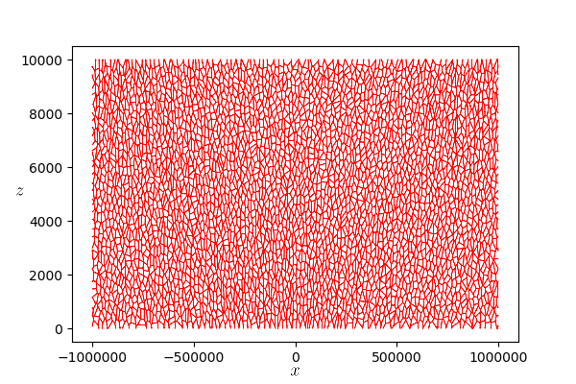
\includegraphics[width=0.7\linewidth]{evaluation/laguerre_tesselation_5}}}
	\caption{Plot of Laguerre Cells generated using a random mesh of $80 \times 40$ points initialised in geostrophic space using \ref{Initpoints} at (a) $0$ days and (b) $2.5$ days , $\Gamma = [-L,L]\times[0,H]$, where $L = 1\times10^6$ and $H = 1\times10^4$}
	\label{lagcells1}
\end{figure}
\newpage
\begin{figure}[h!]
	\centering
	\subfloat[]{{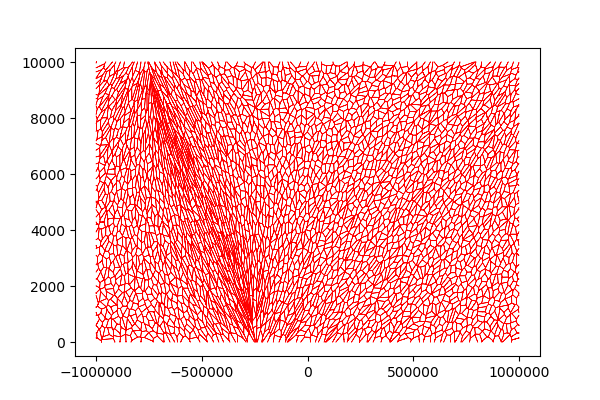
\includegraphics[width=0.7\linewidth]{evaluation/laguerre_tesselation_12}}}\\
	\subfloat[]{{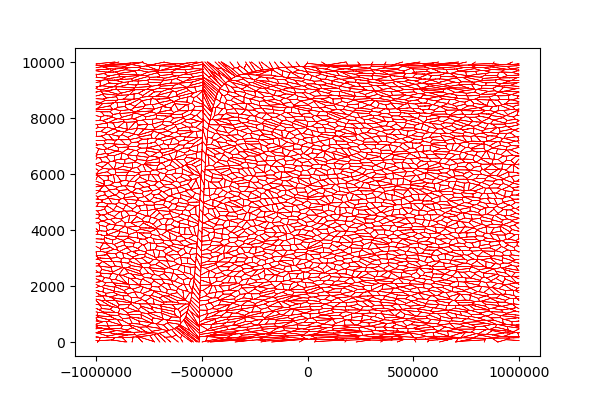
\includegraphics[width=0.7\linewidth]{evaluation/laguerre_tesselation_18}}}
	\caption{Plots of Laguerre Cells generated using a random mesh of $80 \times 40$ points initialised in geostrophic space using \ref{Initpoints} at (a) $6$ days (b) $9$ days $\Gamma = [-L,L]\times[0,H]$, where $L = 1\times10^6$ and $H = 1\times10^4$}
	\label{lagcells2}
\end{figure}
\newpage
\section{Total Energy as a Measurement of Error \label{energyerror}}
\begin{figure}[h]
	\centering
	\subfloat[]{{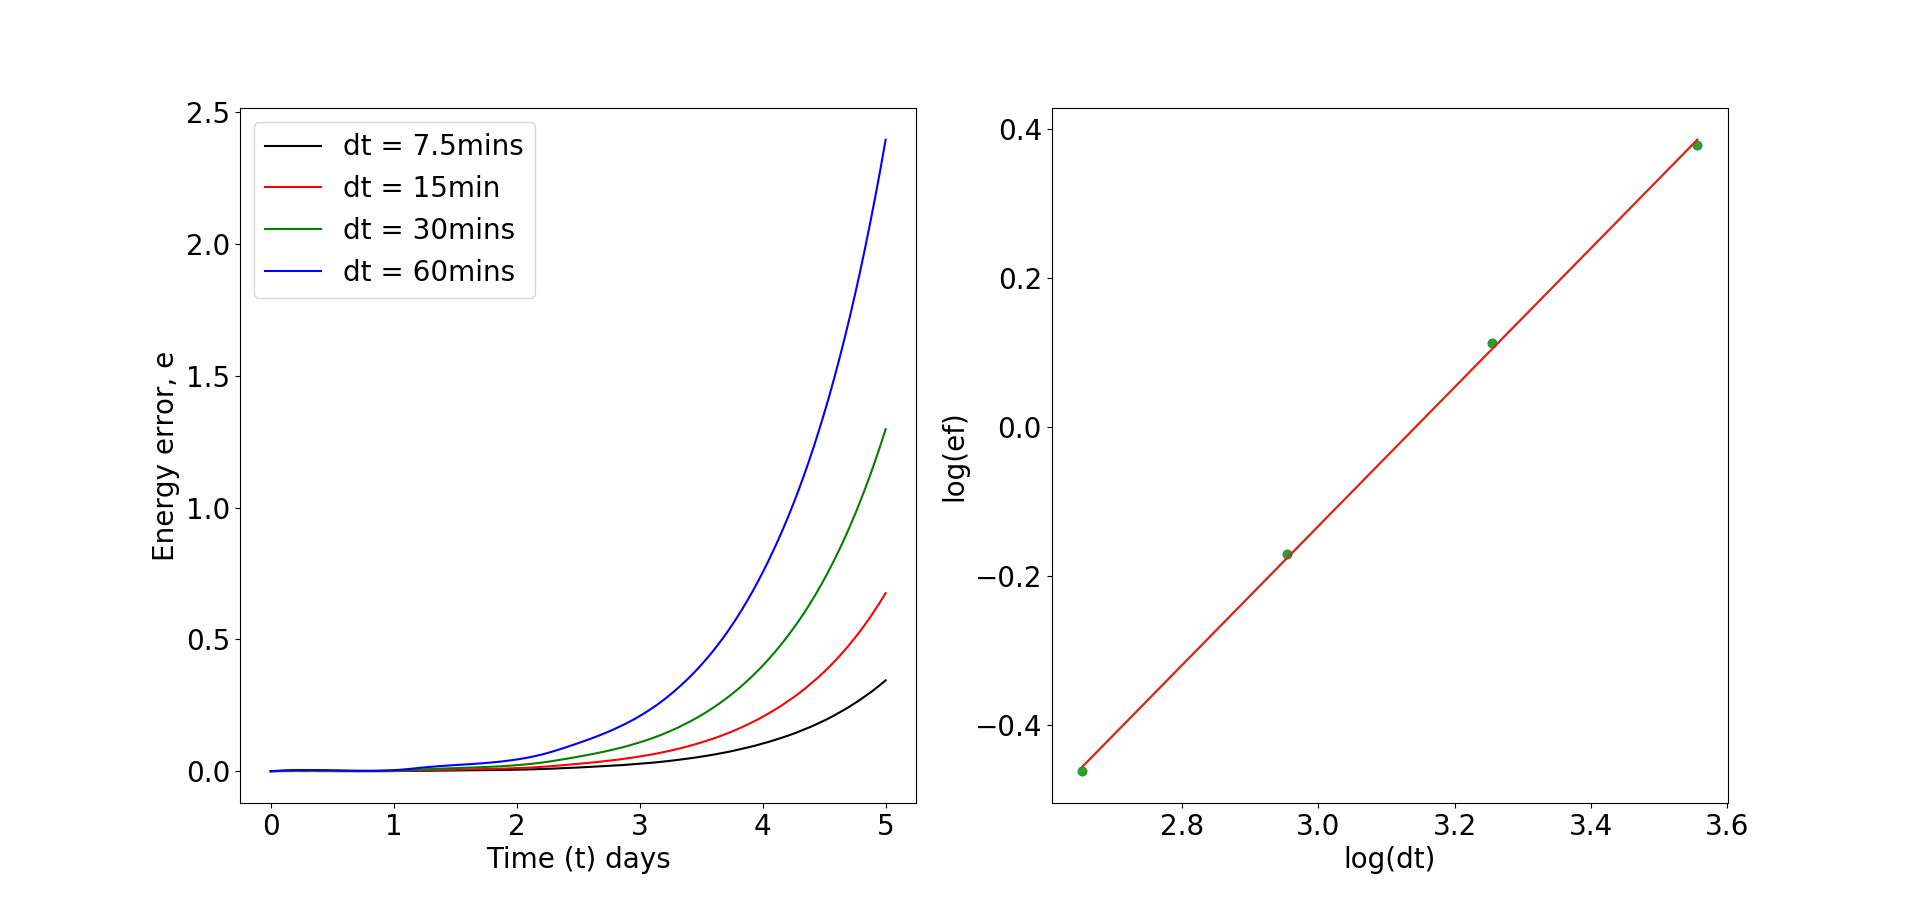
\includegraphics[width=0.9\linewidth]{evaluation/energy_5D_euler}}}\caption[Energy Error from implementation of SG/DA via Forward Euler timestepping method for 5 days]{Energy error following the implementation of SG/DA with a Forward Euler time stepping method for 5 days on a regular mesh of $80 \times 40$ points. $\log(\Delta t)$ vs. $\log(e_f)$. The line of best fit has gradient $m = 0.933$, 3.s.f} \label{fig:energy5deuler}
\end{figure}
\begin{figure}
	\subfloat[]{{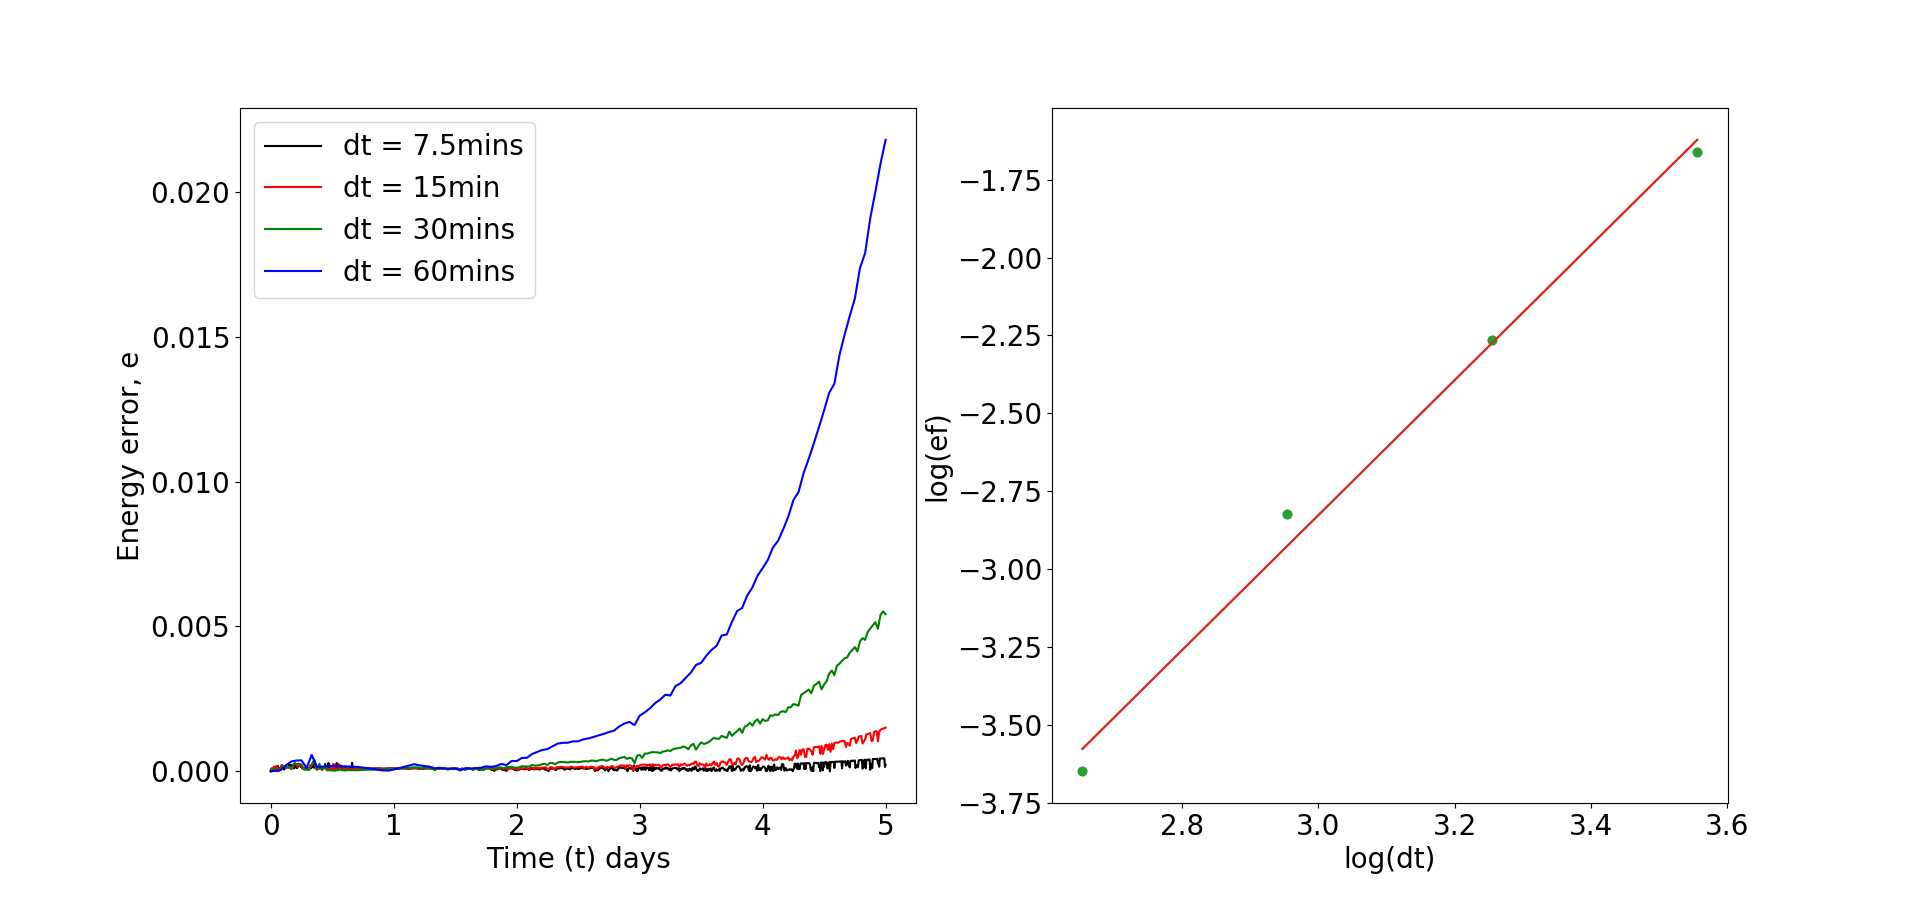
\includegraphics[width=0.9\linewidth]{evaluation/energy_5D_heun}}}\caption[Energy Error from implementation of SG/DA via Heun timestepping method for 5 days]{ Energy error following the implementation of SG/DA with a Heun time stepping method for 5 days on a regular mesh of $80 \times 40$ points. $\log(\Delta t)$ vs. $\log(e_f)$. The line of best fit has gradient $m = 2.17$, 3.s.f}
	\label{fig:energy5dheun}
\end{figure}
The aim of this section is to validate the results seen in section \ref{laguerre plots} above. With no known analytical solutions to the Eady model for frontogenesis \ref{EadyModel} that we are studying and with no numerical models achieving the resolution we are able to achieve with SG/DA a challenge arises in how to confirm that the results are suitable solutions for the Semi-geostrophic Eady model. In this case, we turn to the total energy to quantify the error in the implementation. This is justified as we know from \cite{Cullen2006a} that the total energy in equation \ref{EadyModel} is conserved. However, given the form of total energy from \ref{energy} as,

\begin{equation}
	E = f^2 \iint \frac{1}{2}\left(X-x\right)^2 - Z\left(z - H/2\right)\textrm{d}x\textrm{d}z
\end{equation}

There is a clear dependence on the values of the points in geostrophic space and the values of the centroids of their corresponding Laguerre cells. This indicates a dependence of the total energy of the system on the numerical solution given by SG/DA at each time-step. The graphs below show the total energy given by a system initialised from a grid of $80 \times 40$ points in geostrophic space (again from applying the transformation to points in physical space by \ref{Initpoints}). This time a regular mesh was used to ensure that the initial energy ($E_0$) was the same for each simulation. \\
\linebreak
The effect of decreasing the time step value was investigated for  both the Forward Euler and Heun time stepping schemes. In the following plots the energy error, $e_t$ is defined as $e_t = E_{t} - E_0$. The final energy error $e_f$ is used to create log-log plots confirming the relationship between the time step used and the numerical error of the implementation. What is most interesting in this is the gradient of the line of best fit, this gives an indication of the order of accuracy of the method. What we expect to see is a gradient, $m$, close to $m=1$ for the Euler method as this is well known to have a linear rate of converge \cite{Griffiths2010} and $m=2$ for the Heun method as this has a quadratic rate of convergence \cite{Griffiths2010}.
\newpage


\newpage

Figures \ref{fig:energy5deuler} and \ref{fig:energy5dheun} indicate promising initial findings. The straight lines in the log-log plots are clear evidence of a power law governing the error - time step relation. Moreover, the gradient values are reasonably close to what we were expecting.\\
\linebreak
The difference in computed values for the gradient to expected values is attributable to the error in applying the Damped Newton Algorithm in DA. To expand, rates of convergence are computed assuming $f(t,\bm{x})$ in $\frac{\textrm{d}\bm{x}}{\textrm{d}t} = f(t,\bm{x})$ has a Taylor expansion \cite{Griffiths2010}. In the case of SG/DA the right hand side includes the implementation of DA which carries error associated with the Damped Newton Algorithm. This is particularly visible in the Heun implementation where the error is significantly smaller. In this case the error associated with DA dominates that associated with the Heun's method and is seen as noise in the energy error curve.\\
\linebreak
Physically we can see that the energy error begins to grow the most between days $4$ and $5$, which coincides with the point where the front seen in figures \ref{fig: thetap ldiag1},\ref{fig: thetap ldiag2} begins to grow most rapidly. To investigate this further the energy error is found for a period of up to $10$ days.
\newpage
\begin{figure}[ht]
	\centering
	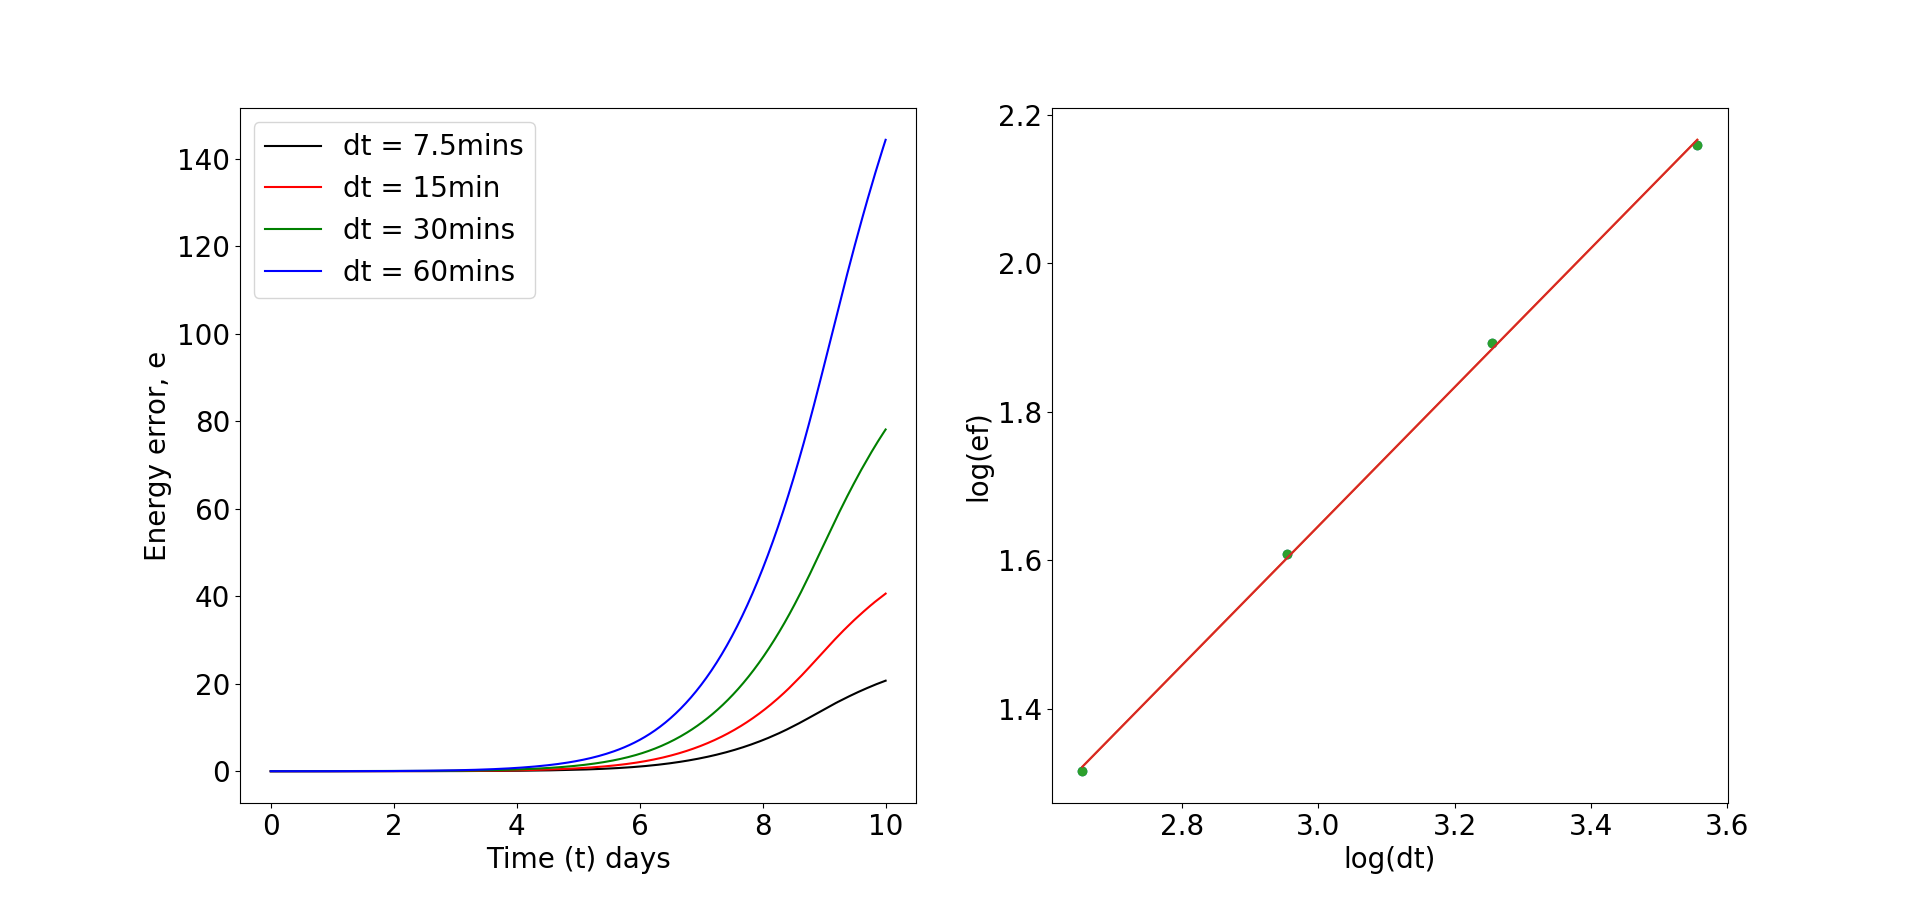
\includegraphics[width=1.1\linewidth]{evaluation/energy_10D_euler}
	\caption[Energy Error from implementation of SG/DA via Forward Euler timestepping method for 10 days]{(a) Energy error following the implementation of SG/DA with a Forward Euler time stepping method for 10 days on a regular mesh of $80 \times 40$ points.\\ (b) $\log(\Delta t)$ vs. $\log(e_f)$. The line of best fit has gradient $m = 0.935$, 3.s.f}
	\label{fig:energy10deuler}
\end{figure}
\begin{figure}[h]
	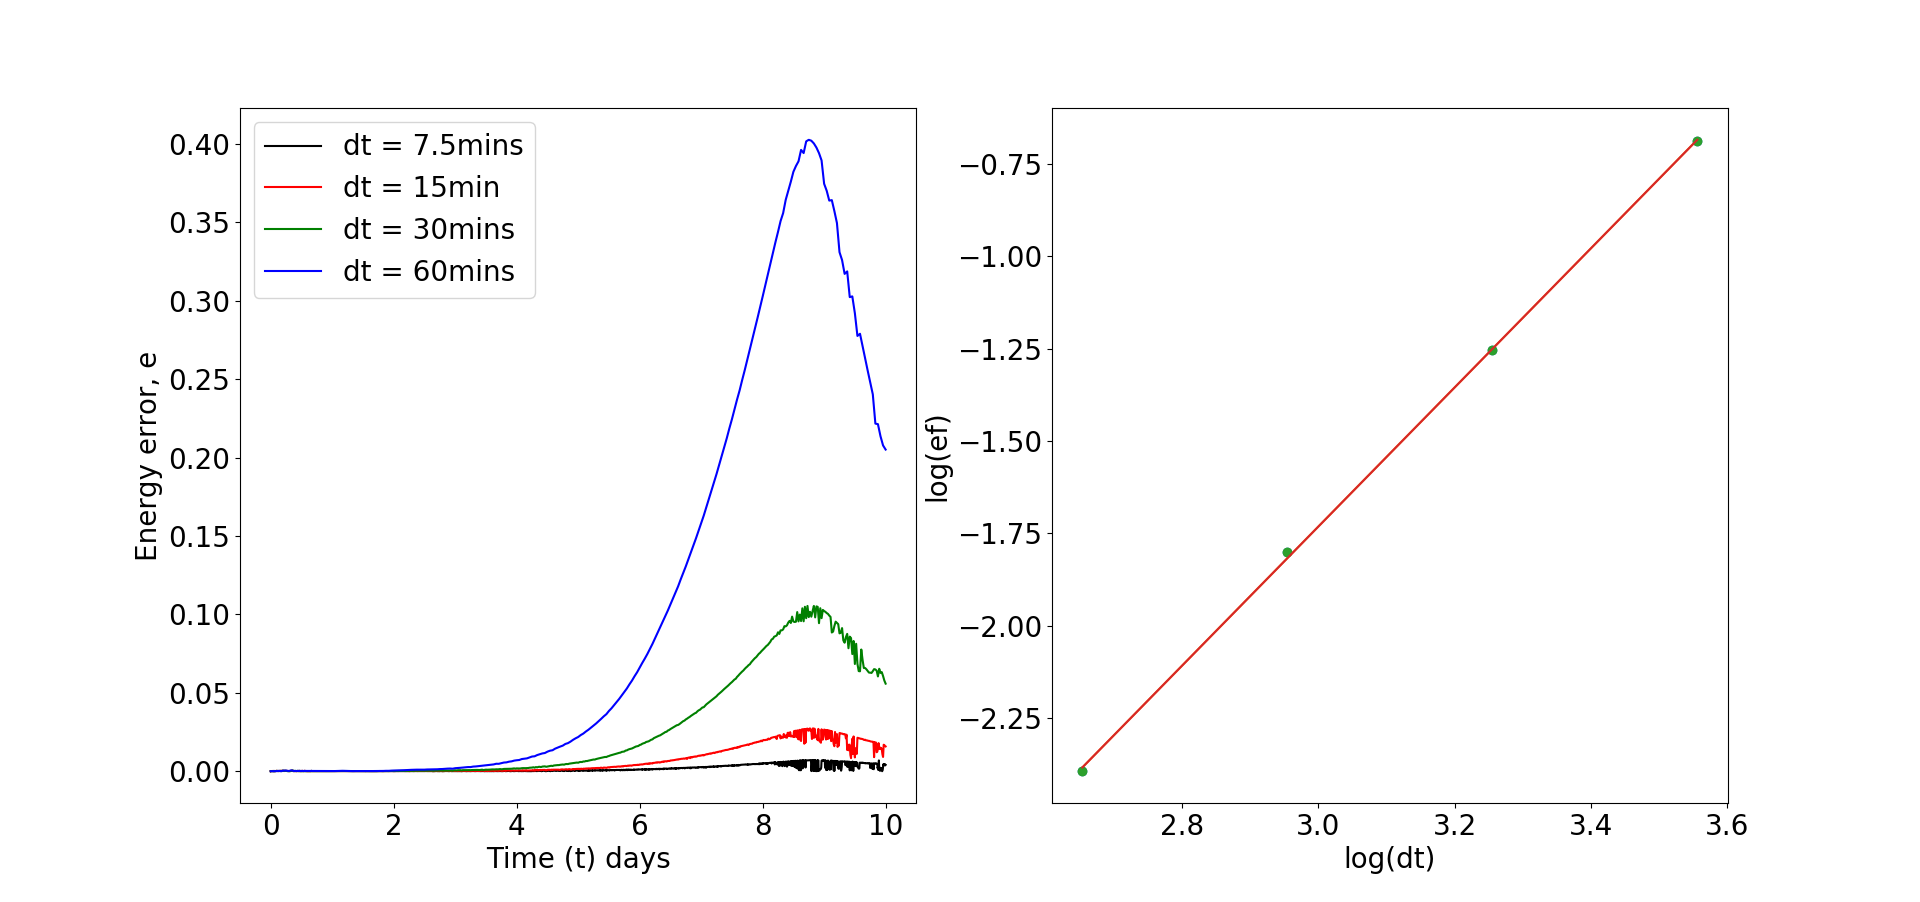
\includegraphics[width=1.1\linewidth]{evaluation/energy_10D_heun}
	\caption[Energy Error from implementation of SG/DA via Heun timestepping method for 10 days]{(a) Energy error following the implementation of SG/DA with a Heun time stepping method for 10 days on a regular mesh of $80 \times 40$ points.\\ 
		(b) $\log(\Delta t)$ vs. $\log(e_f)$. The line of best fit has gradient $m = 1.88$, 3.s.f}
	\label{fig:energy10dheun}
\end{figure}  
\pagebreak
\section{A Comparison of Time Stepping Methods \label{comparison}}

\begin{figure}[h]
	\centering
	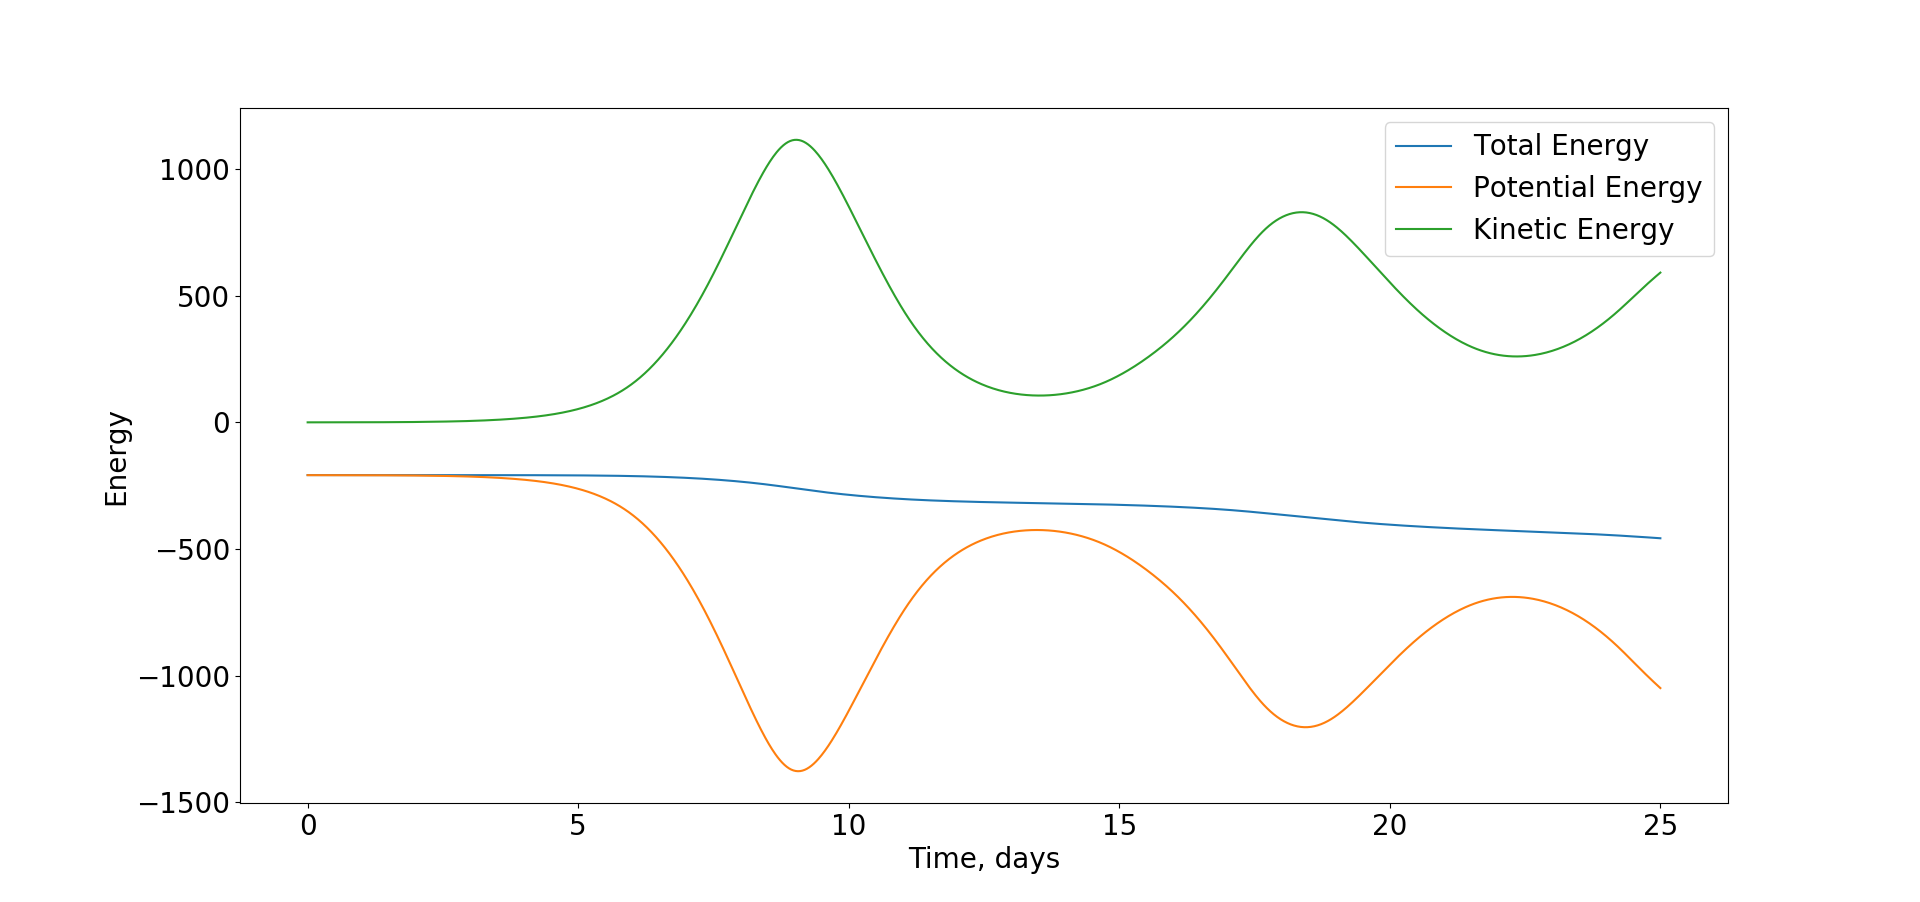
\includegraphics[width=0.8\linewidth]{evaluation/Energy_evolution_euler}
	\caption[Energy evolution for SG/DA with Euler time step scheme]{Energy evolution for SG/DA with Euler time step scheme for regular grid of initialised points}
	\label{fig:energyevolutioneuler}
\end{figure}

To validate the behaviour exhibited in section \ref{laguerre plots} we look at the behaviour of the Kinetic Energy, Potential Energy and Total Energy with time. We restate the energy in the form \ref{energy},

\begin{equation}
	E= f^2 \iint \frac{1}{2}\left(X-x\right)^2 - Z\left(z - H/2\right)\textrm{d}x\textrm{d}z
\end{equation}

The kinetic energy over the domain $\Gamma$ is defined by,

\begin{equation}
	E_{kin} = \int_\Gamma \ \frac{f^2}{2}(X-x)^2 \ dxdz
\label{KE}
\end{equation}

And the potential energy given by,

\begin{equation}
E_{pot} = \int_\Gamma \ - Z\left(z - H/2\right) \ dxdz
\label{PE}
\end{equation}

We now investigate the evolution of these quantities for a period of 25 days for each time stepping method, initialised with a regular mesh of $80 \times 40$ points transformed to geostrophic co-ordinates as in \ref{Initpoints}.
In figure \ref{fig:energyevolutioneuler} the cycle of frontogenesis and collapse is much clearer seen in the periodic nature of the Kinetic energy. The graph also shows that energy dissipation in the Forward Euler method is strongest after front formation.

\begin{figure}[h!]
	\centering
	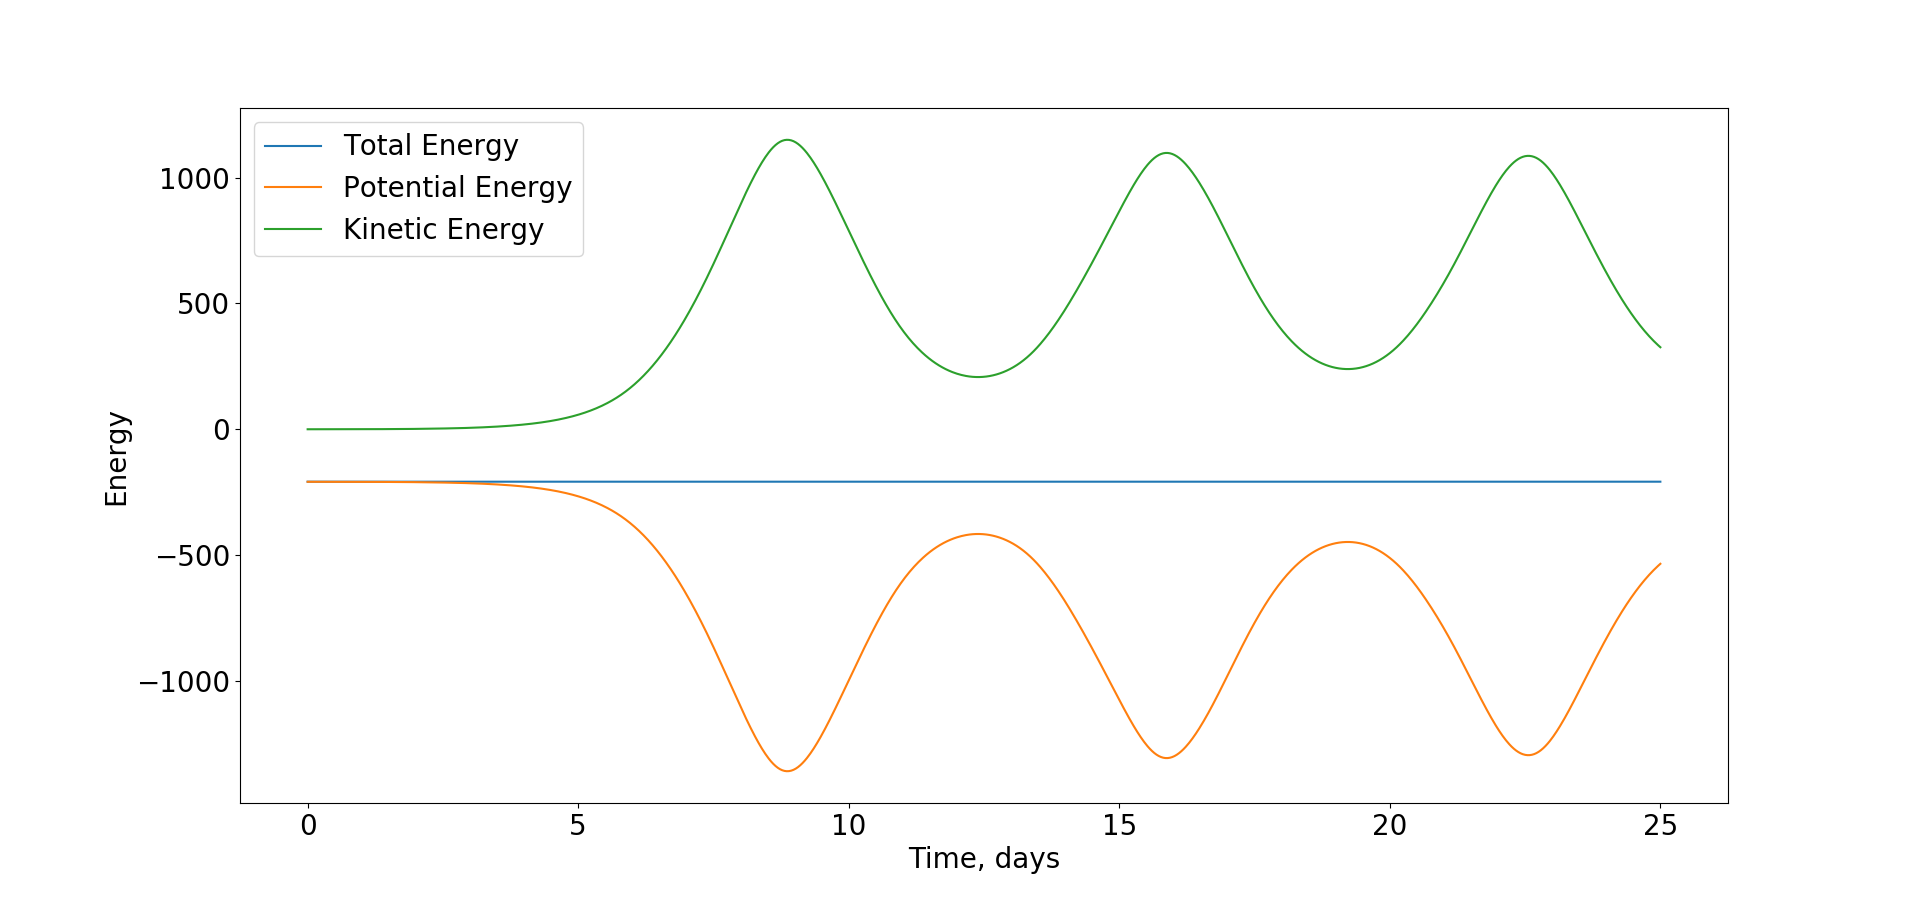
\includegraphics[width=0.8\linewidth]{evaluation/Energy_evolution_heun}
	\caption[Energy evolution for SG/DA with Heun time step scheme]{Energy evolution for SG/DA with Heun time step scheme for an initially regular grid of points}
	\label{fig:energyevolutionheun}
\end{figure}

From figure \ref{fig:energyevolutionheun} we see that Heun's method gives numerical results that appear to maintain energy conservation. Comparing the kinetic energy to that of the Forward Euler method there is significantly less damping in the cycle of front formation. The differences in behaviour of kinetic energy is explored further in \ref{fig:energyeulerheuncomparison}.
\\
\linebreak
The comparison in figure \ref{fig:energyeulerheuncomparison} shows a significant damping in the amplitude of oscillations in the Forward Euler time stepping scheme compared to the Heun scheme, where the second oscillation appears slightly damped but the third very similar in amplitude to the second. What is also striking is the difference in the periods of oscillation. The period of oscillation in Heun's method is significantly smaller and more uniform indicating a dispersion error in the Forward Euler implementation. 
\comments{\cite{Cullen2006a}period of oscillation}
\begin{figure}[h!]
	\centering
	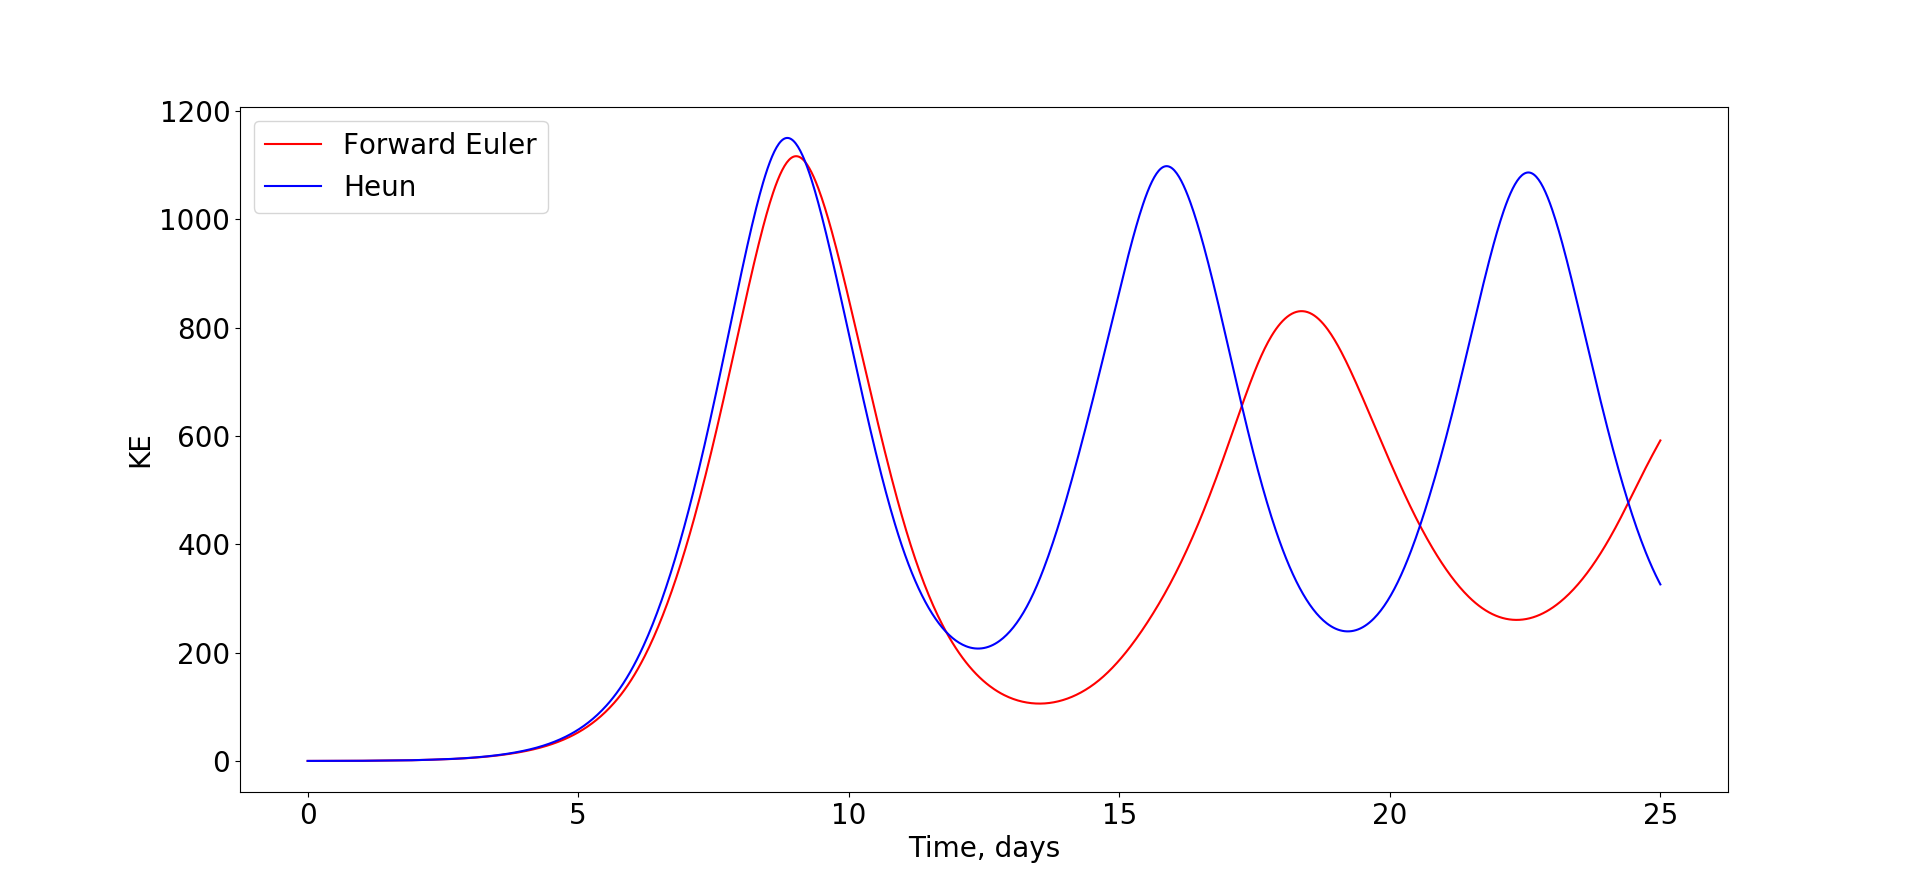
\includegraphics[width=0.9\linewidth]{evaluation/energy_euler_heun_comparison}
	\caption[Comparison of Energy Evolution for SG/DA with Heun/Forward Euler Time Stepping Schemes]{Comparison of energy evolution of solution of SG/EM with SG/DA for Heun and Forward Euler time-stepping schemes over a period of 25 days with a regular grid of initial points}
	\label{fig:energyeulerheuncomparison}
\end{figure}

\newpage
\section{Computational Performance}
The results of sections \ref{comparison} and \ref{energyerror} show a clear indication that using Heun's method for the time stepping of SG/DA gives a significantly more accurate result. However, considering that to implement Heun's method requires two calls to DA to solve the optimal transport problem at the prediction stage and correction stage the benefit of extra accuracy could be lost in a large increase to the runtime of the algorithm. Due to this we would expect the runtime of Heun's method to be close to twice that of Euler's method. In this section we investigate the additional time cost to running Heun's method in time stepping and evaluate whether this is justified.

\begin{table}[h!]
	\begin{tabular}{|c|c|c|} 
		\hline 
		$N$, ($2N^2$ points) & Runtime (s) FE Method & Runtime (s) Heun Method \\ 
		\hline 
		30 & 40.430 & 81.479 \\ 
		\hline 
		35 & 59.898 & 114.232 \\ 
		\hline 
		40 & 93.374 & 179.741 \\ 
		\hline 
		45 & 148.440 & 274.582 \\ 
		\hline 
		50 & 200.886 & 372.805 \\ 
		\hline 
		55 & 286.968 & 503.502 \\ 
		\hline 
		60 & 410.417 & 663.437 \\ 
		\hline
	\end{tabular}
\caption[Comparison of Runtime by Forward Euler and Heun's time step methods]{A comparison of runtime (seconds) by Forward Euler and Heun's time step methods using python cProfile package}
\label{table: runtime}
\end{table}

To compare the runtime of each time stepping method the python package cProfile was used around the time iteration part of the algorithm. Of course, this means that some set-up time costs are factored into the runtime measurement. From table \ref{table: runtime} it is already evident from table that the runtime of Heun's method is significantly greater than that of the Forward Euler method. Whilst for smaller values of $N$ the runtime is approximately doubles between implementing Euler and Heun's method we see that above $N = 45$ this relationship deteriorates.
\\
\linebreak 
To analyse this further we visualise the data from \ref{table: runtime} by plottin a best fit line for each method by linear regression using the \textquoteleft scipy.stats\textquoteright \ package available in python. 
\begin{figure}[h!]
	\centering
	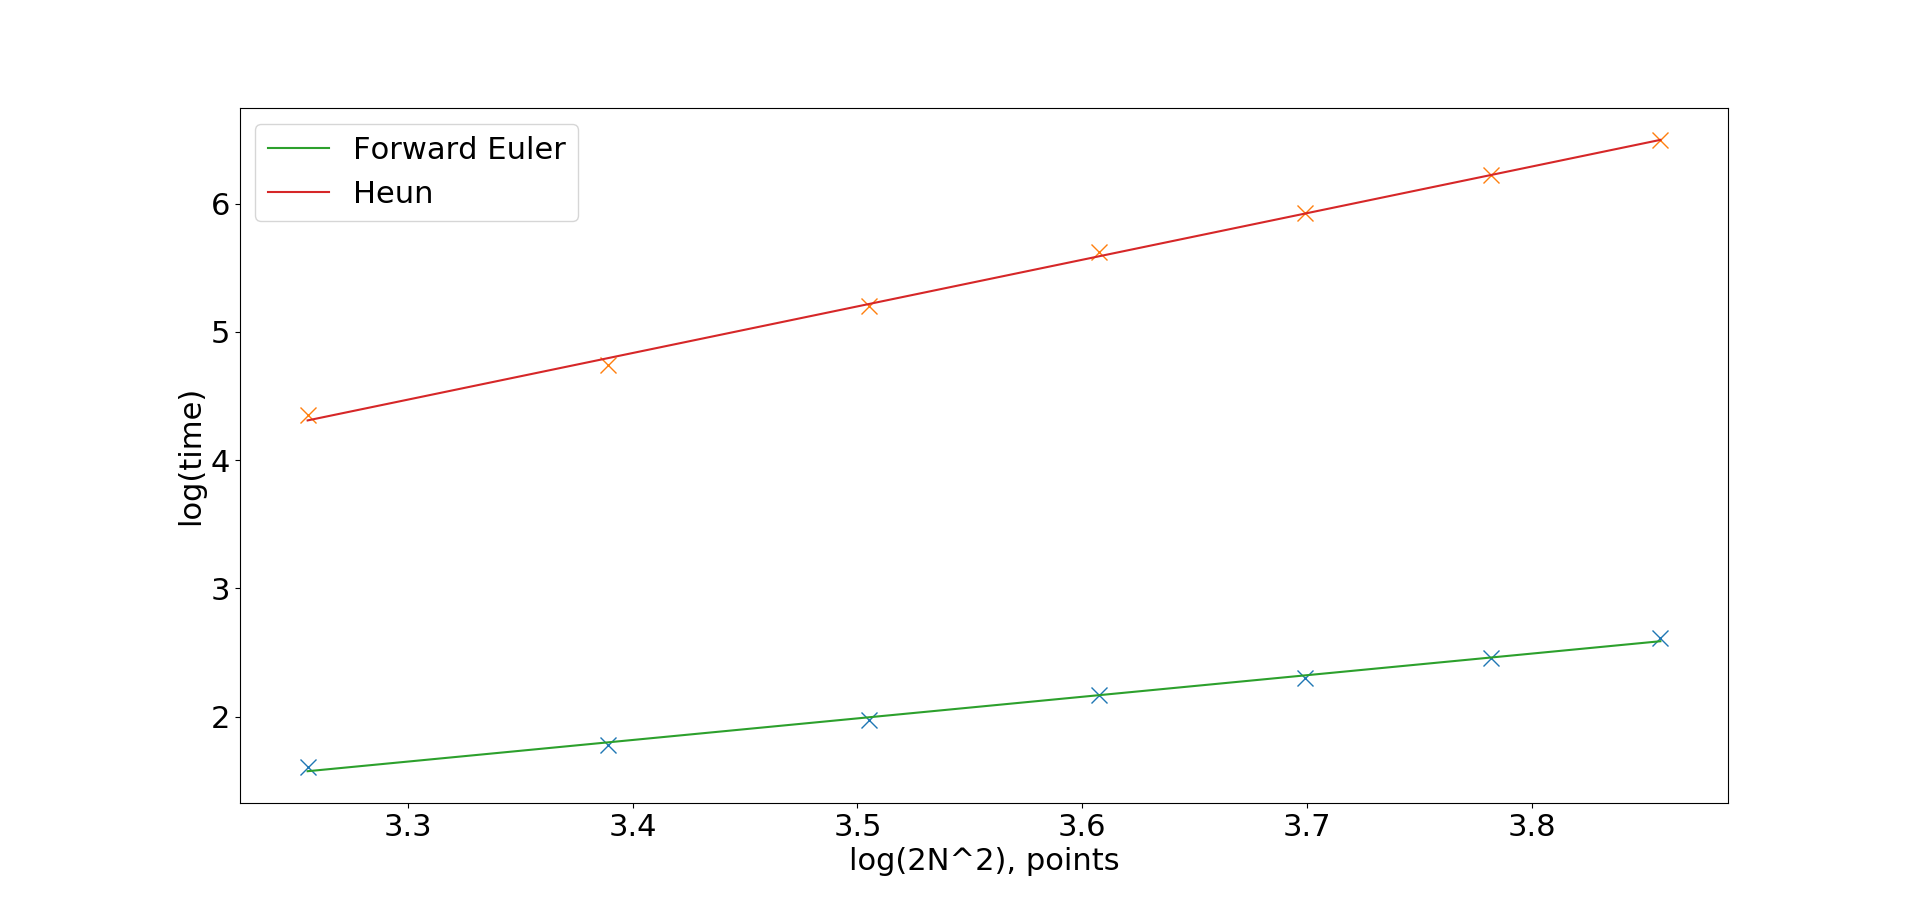
\includegraphics[width=0.95\linewidth]{evaluation/performance_loglog_plot}
	\caption[Time stepping performance based on number of points initialised in the domain]{Logarithmic plot showing $\log(2N^2)$ vs $\log(\textrm{runtime})$ for $N = (30,35,40,45,50,55,60)$ as in table \ref{table: runtime} and line of bestfit. The gradient of the line of bestfit for the Forward Euler method is $1.68$ 3.s.f and for $3.63$ 3.s.f for Heun's method using runtimes from \ref{table: runtime}}
	\label{fig:performanceloglogplot}
\end{figure}
\\
\linebreak
Figure \ref{fig:performanceloglogplot} highlights this disparity observed in the table we see that the gradient in the line of best fit of Heun's method is in fact $2.16$ times that of the Forward Euler method. Indicating another source of time cost in Heun's method. There are a number of reasons this could be. The additional time step calculation for the correction step of Heun's method would contribute to the increase in time cost. 
\\
\linebreak
From the cProfile results, which can be seen from running \textquoteleft SG\_DA\_performance.py \textquoteright \ (in the sg\_monge\_ampere repository) that the greatest time cost is in running DA to solve the optimal transport problem. This runtime could be reduced by recycling the weights from the previous time step as an initial guess for DA in the following time step. In practice this is harder to implement as the time stepping moves points in geostrophic space in the $Z$ direction. This means that the necessary condition for convergence, that the area of the cell associated with each geostrophic point is positive over the domain $\Gamma$ is not necessarily satisfied. Therefore the initial guess given by \ref{Initweights}  must be used for each call to DA. As the initial guess is most likely far from the final values of the weights this will greatly increase the time for DA to converge. As this is called twice in Heun's method this represents an additional cost to runtime which is not so easily quantified. A possible remedy for this is to perturb the values for the weights from the previous time step in such a way that the condition for initial positive cell area is satisfied. However, this is a non trivial problem.